\chapter{Relational Database Service (RDS)}\label{ch:relational-database-service}
% Evie was here…
Amazon RDS service allows a user to create a fully-featured and highly-available SQL database that is automatically
replicated to another availability zone. (TODO: Oops, no multi-az) This means that if the primary database becomes
unavailable, there is automatic failover providing redundancy for all the data stored within.

To create an Amazon RDS instance, a suitable name/identifier for the database is required before created as well as a
selection for the resource limits for the virtual server.
The database requires a username and passphrase, although for additional security there is the option to automatically
generate a passphrase.

Afterwards, the type of SQL database required (such as MySQL, PostgreSQL, MariaDB or others) will be selected and then
the database should begin provisioning.

\begin{figure}[!htbp]
    \centering
    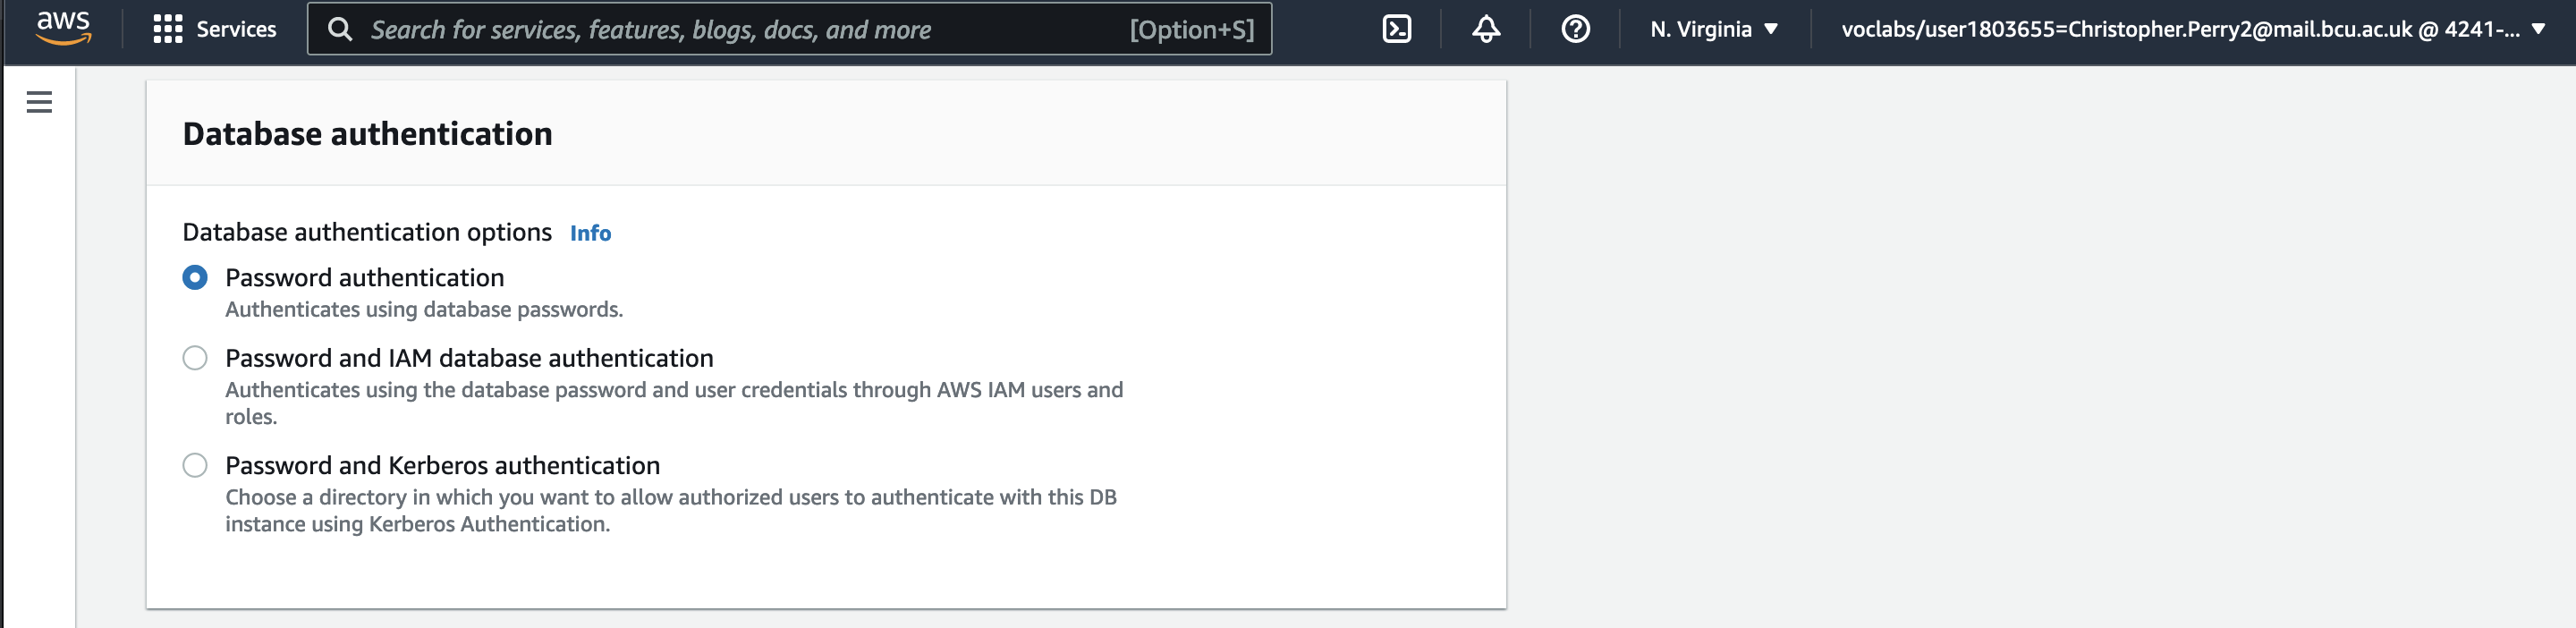
\includegraphics[width=\textwidth]{resources/rds/rds-authentication.png}
    \caption{Selection of CloudWatch metric for EC2 instance.}
    \label{fig:rds-auth}
\end{figure}

\begin{figure}[!htbp]
    \centering
    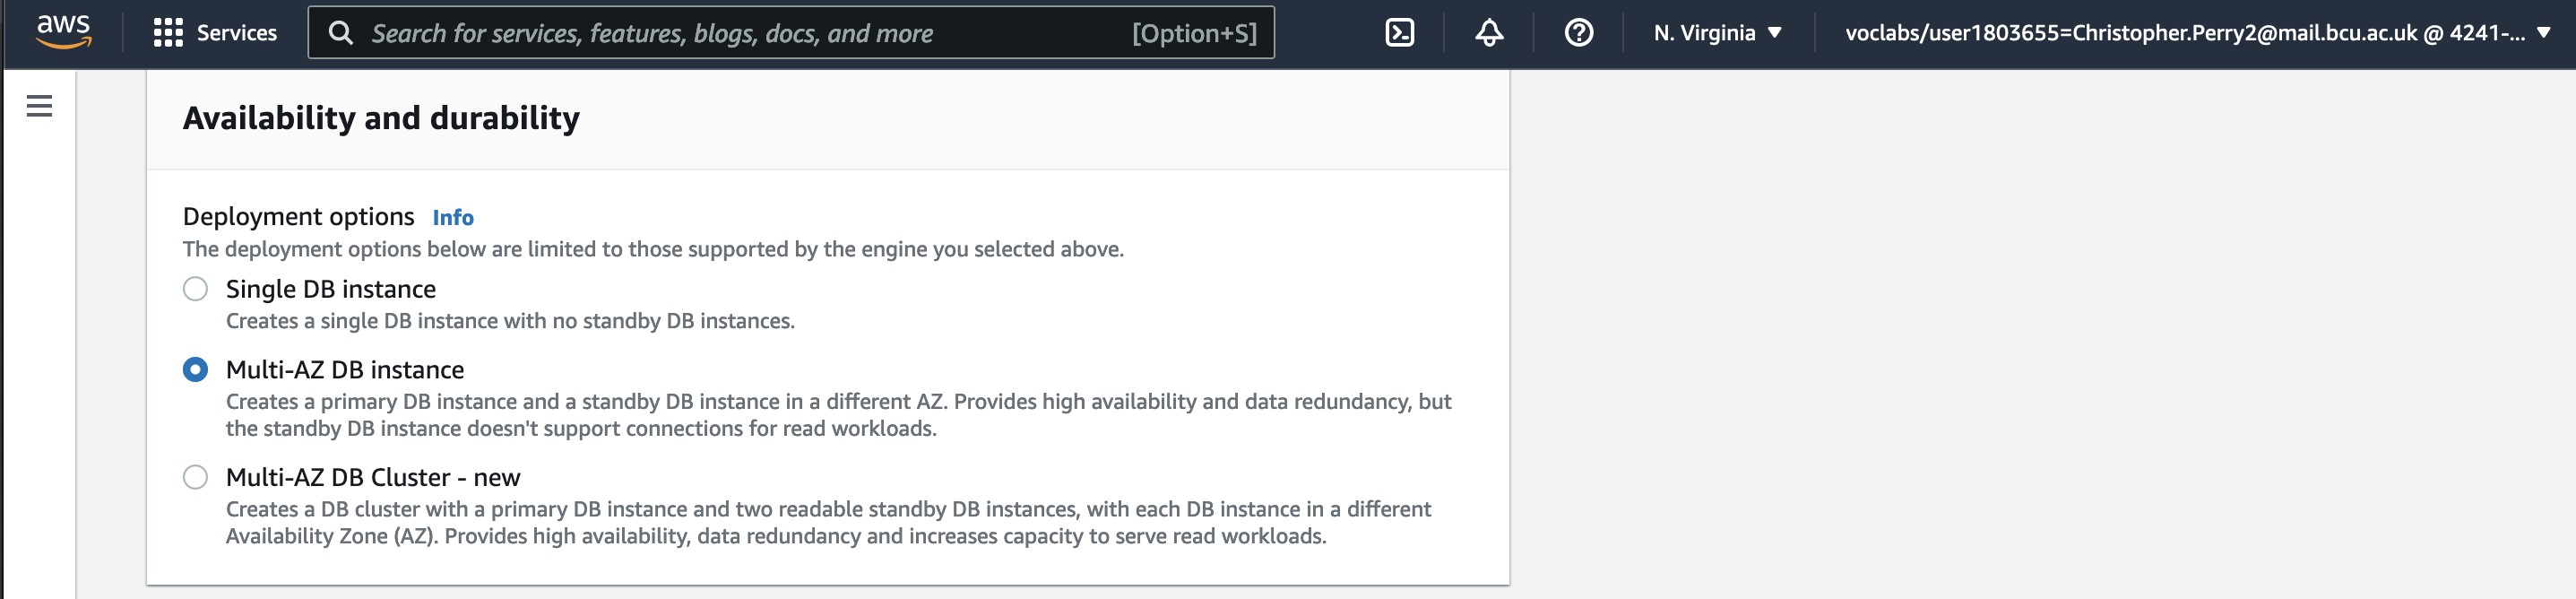
\includegraphics[width=\textwidth]{resources/rds/rds-availability-durability.png}
    \caption{Selection of CloudWatch metric for EC2 instance.}
    \label{fig:rds-avail}
\end{figure}

\begin{figure}[!htbp]
    \centering
    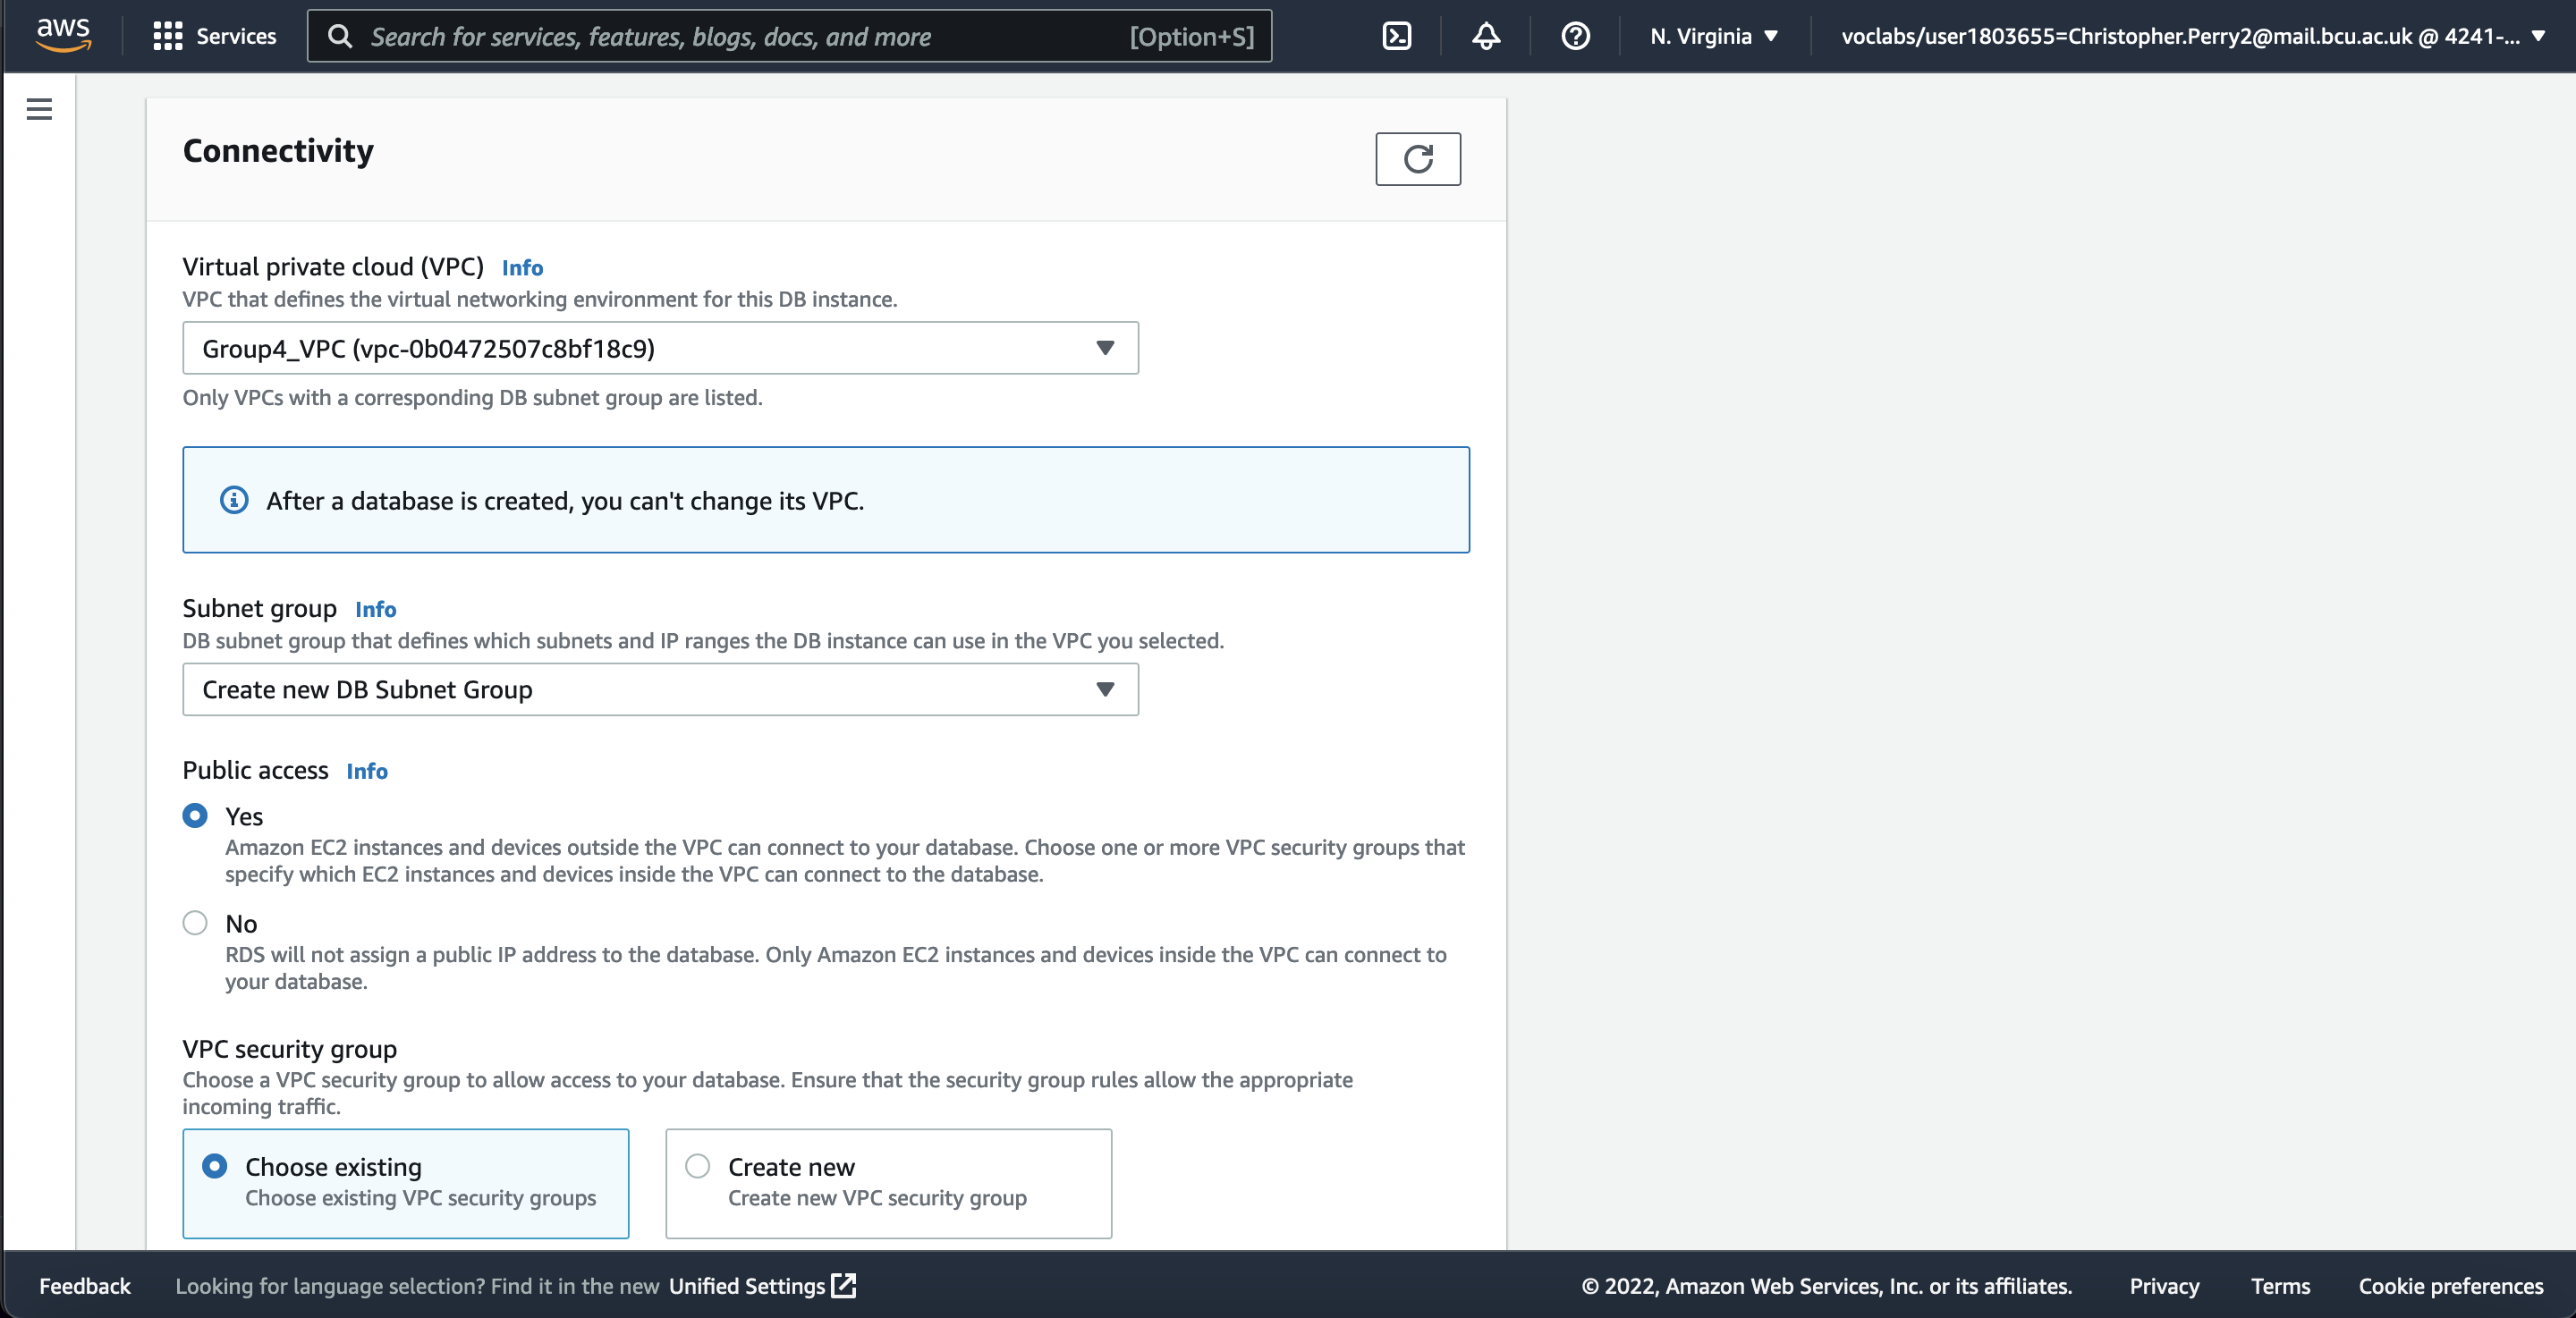
\includegraphics[width=\textwidth]{resources/rds-connectivity-1.png}
    \caption{Selection of CloudWatch metric for EC2 instance.}
    \label{fig:rds-connect}
\end{figure}

\begin{figure}[!htbp]
    \centering
    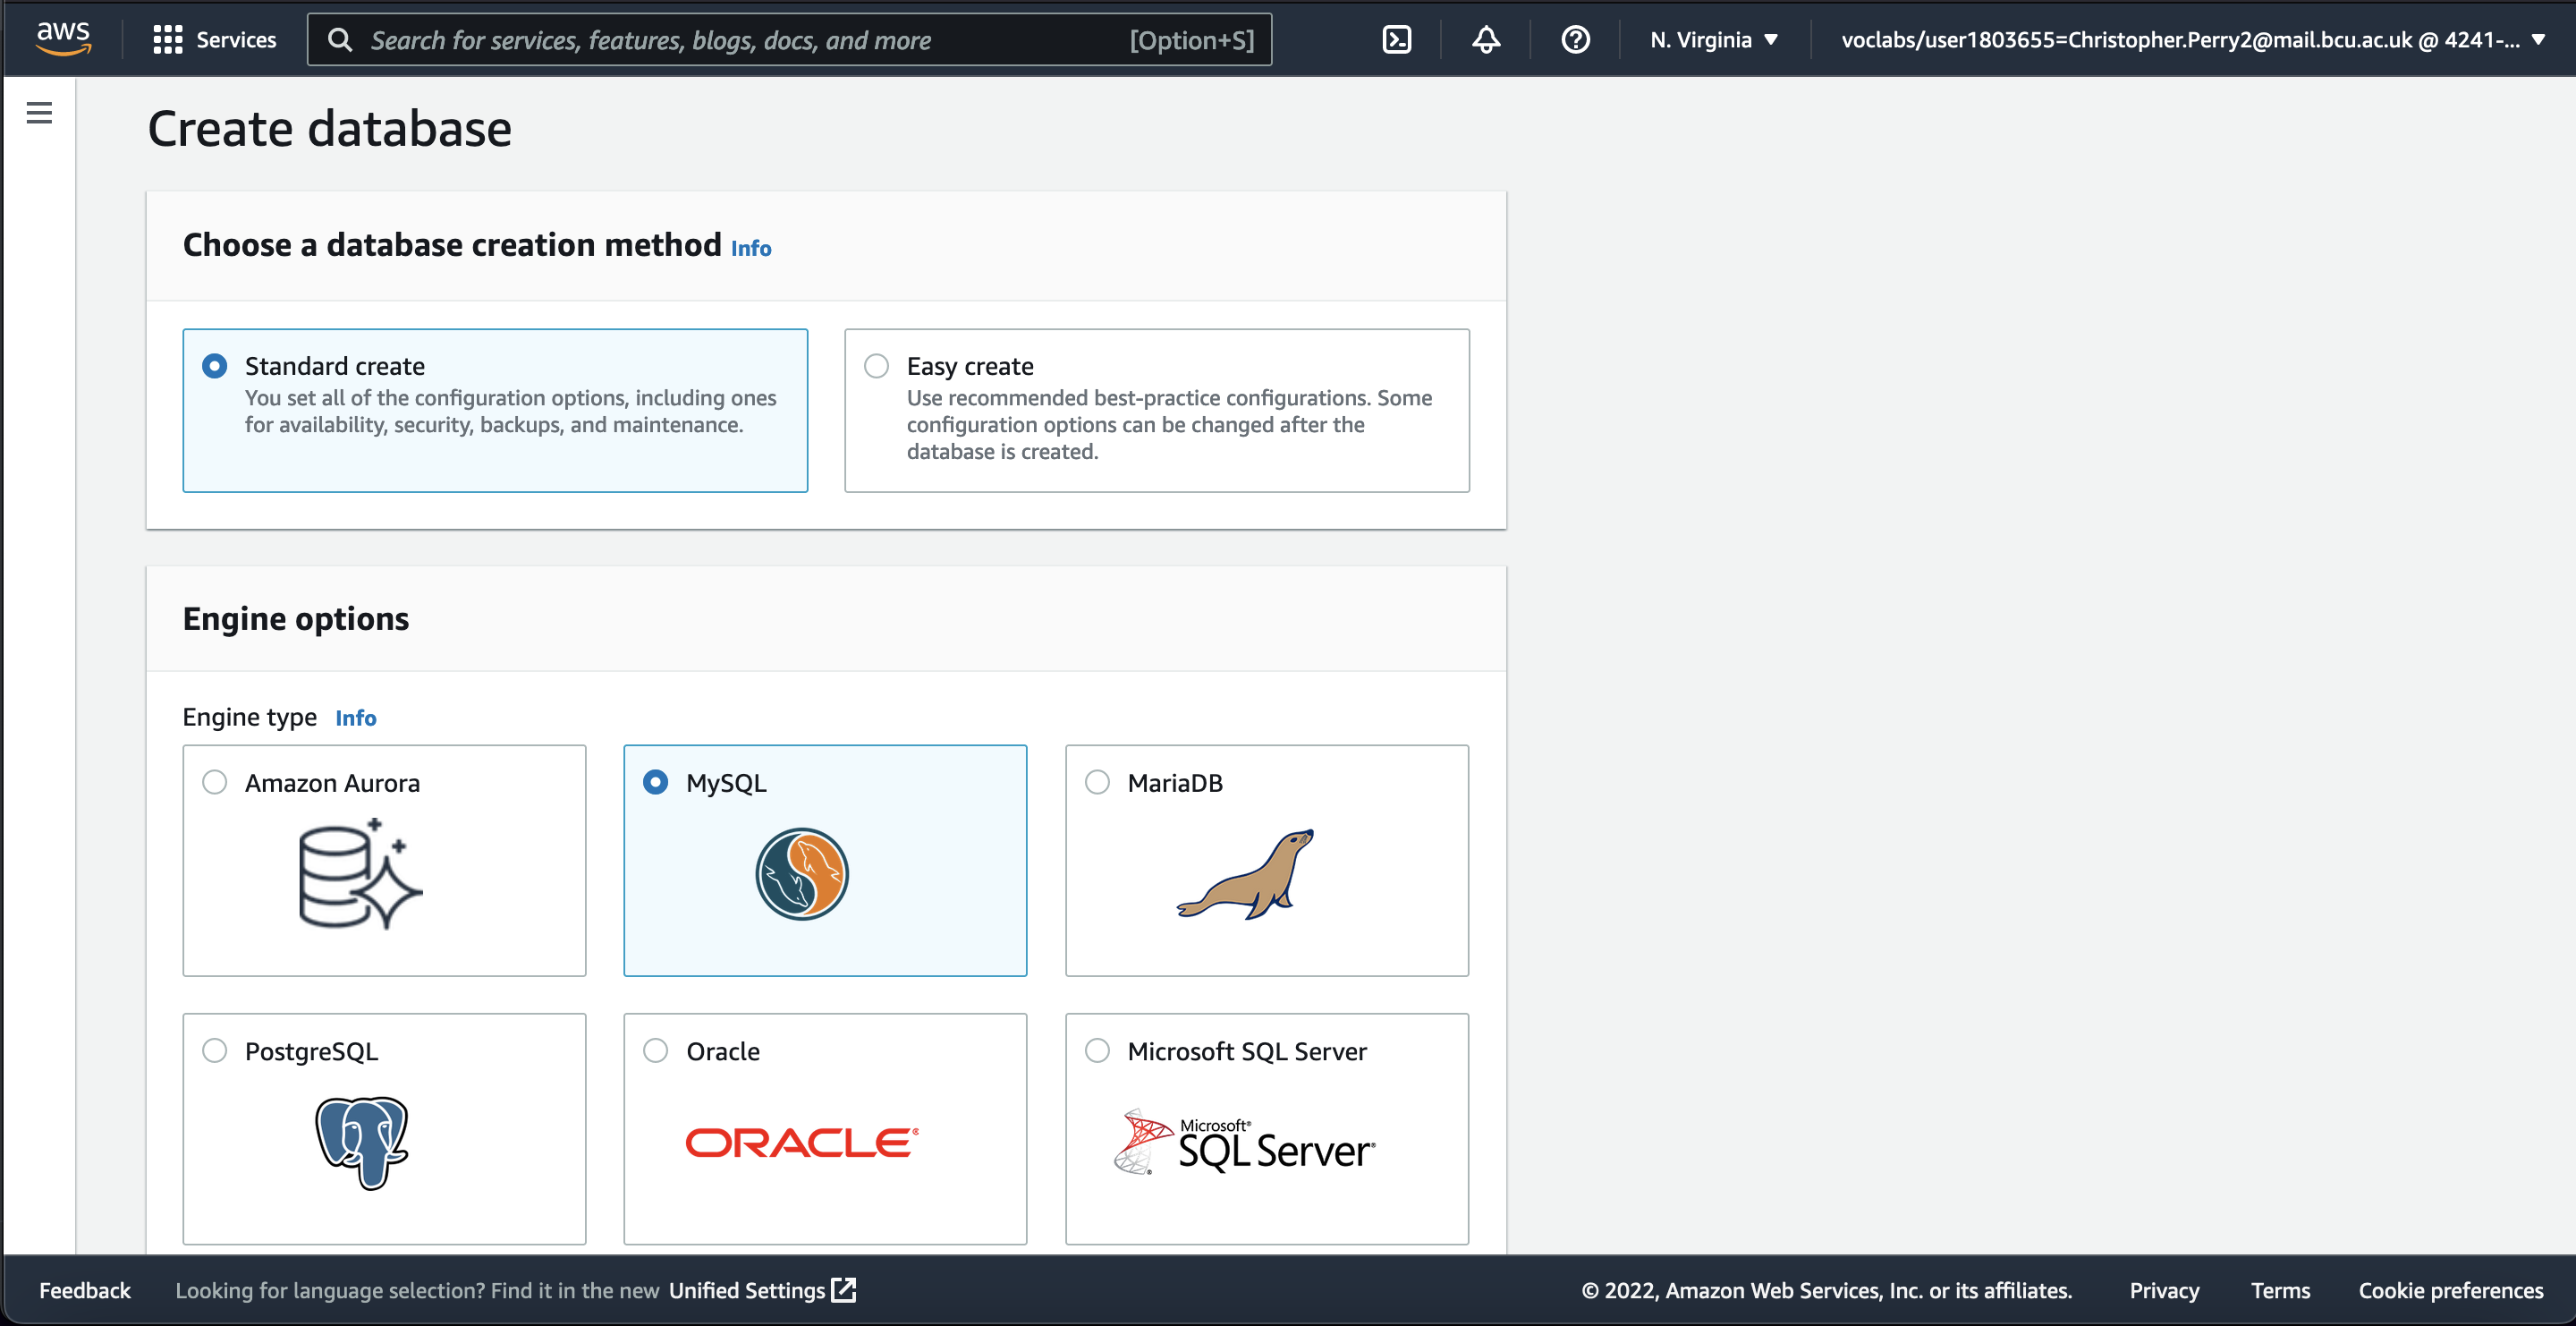
\includegraphics[width=\textwidth]{resources/rds/rds-create-engine.png}
    \caption{Selection of CloudWatch metric for EC2 instance.}
    \label{fig:rds-engine}
\end{figure}

\begin{figure}[!htbp]
    \centering
    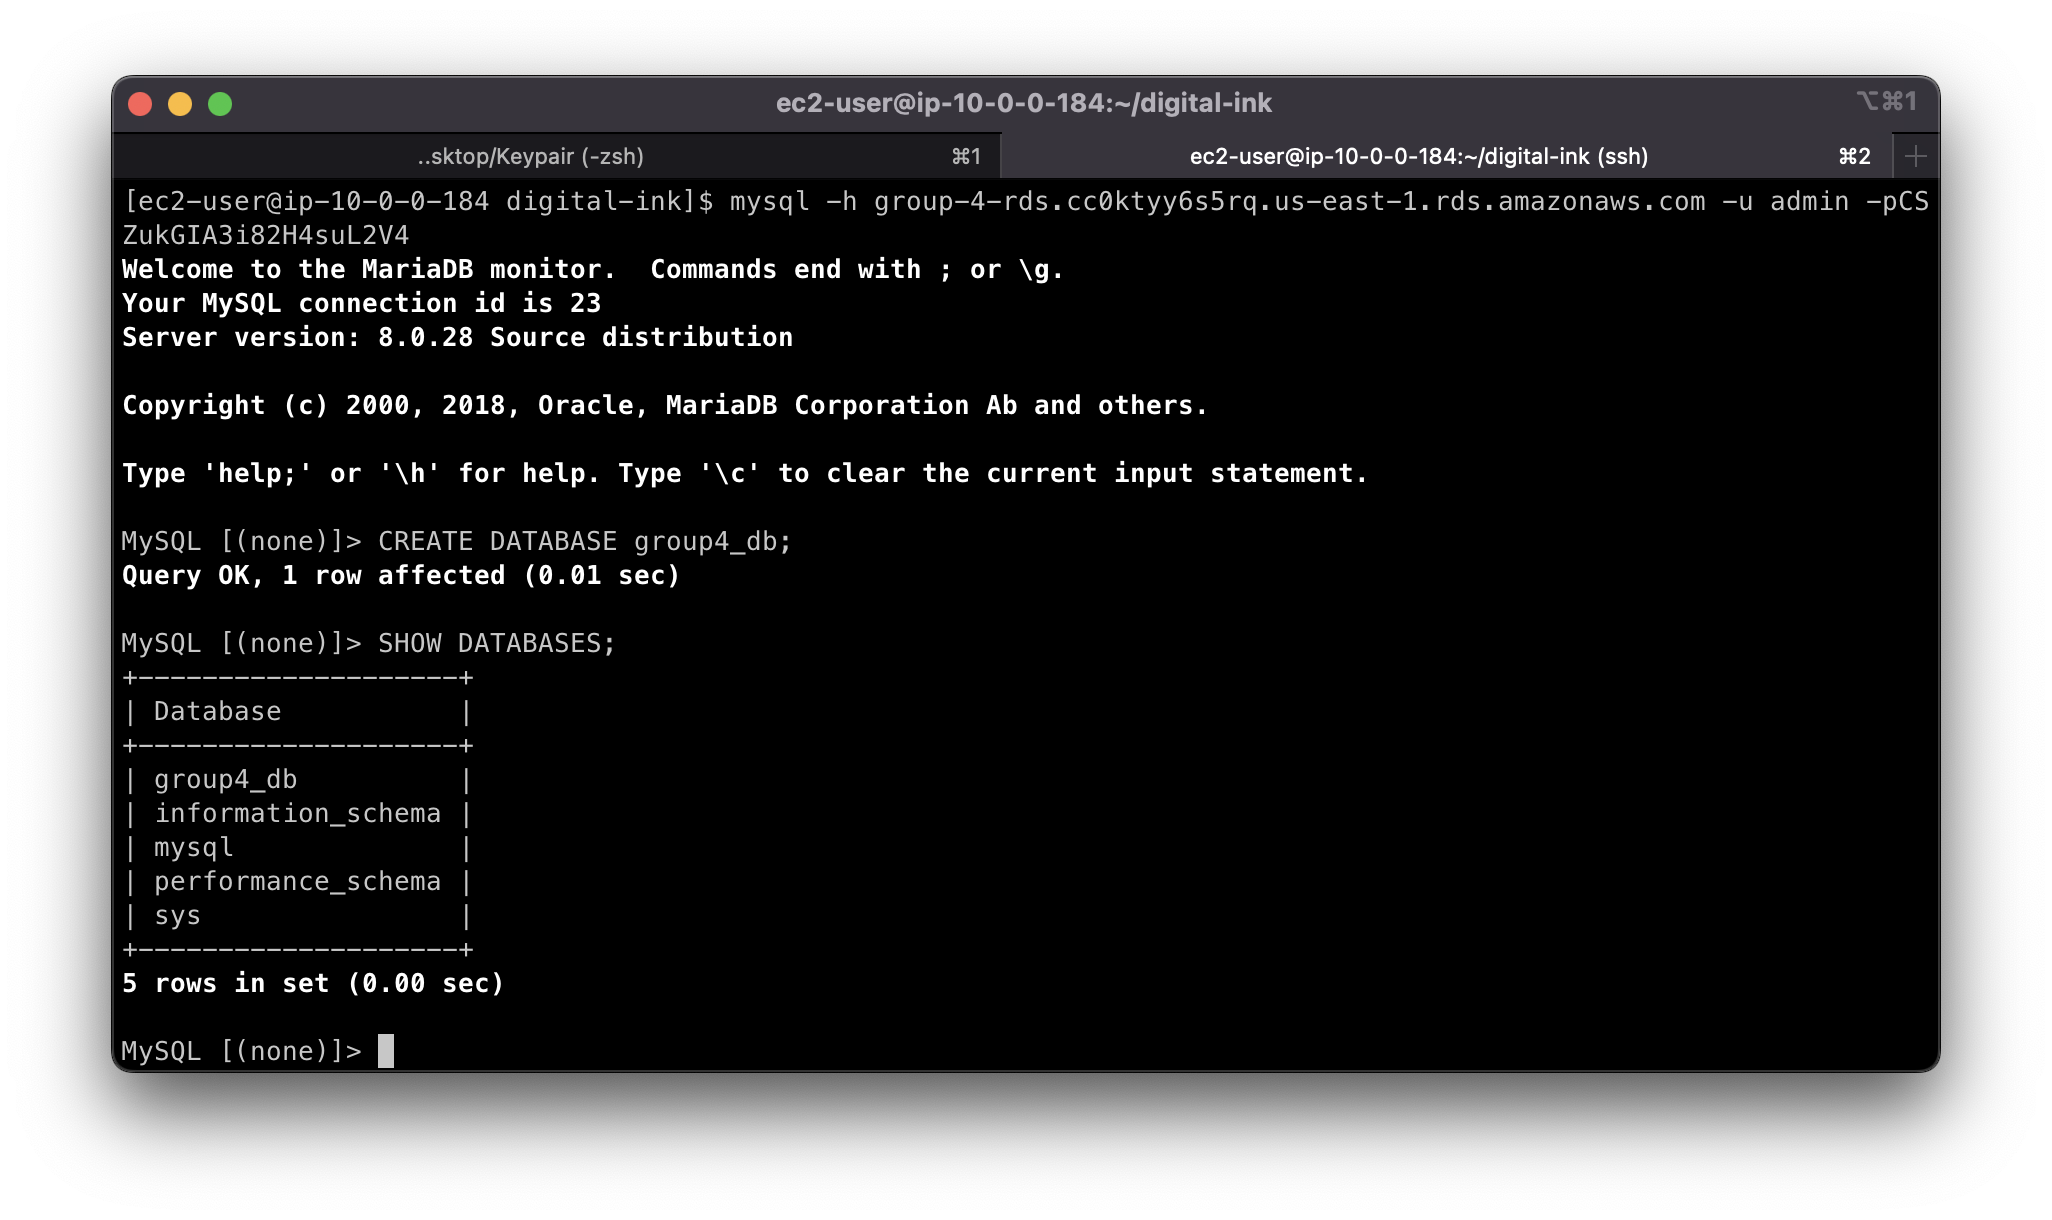
\includegraphics[width=\textwidth]{resources/rds/rds-database-creation.png}
    \caption{Selection of CloudWatch metric for EC2 instance.}
    \label{fig:rds-db-create}
\end{figure}

\begin{figure}[!htbp]
    \centering
    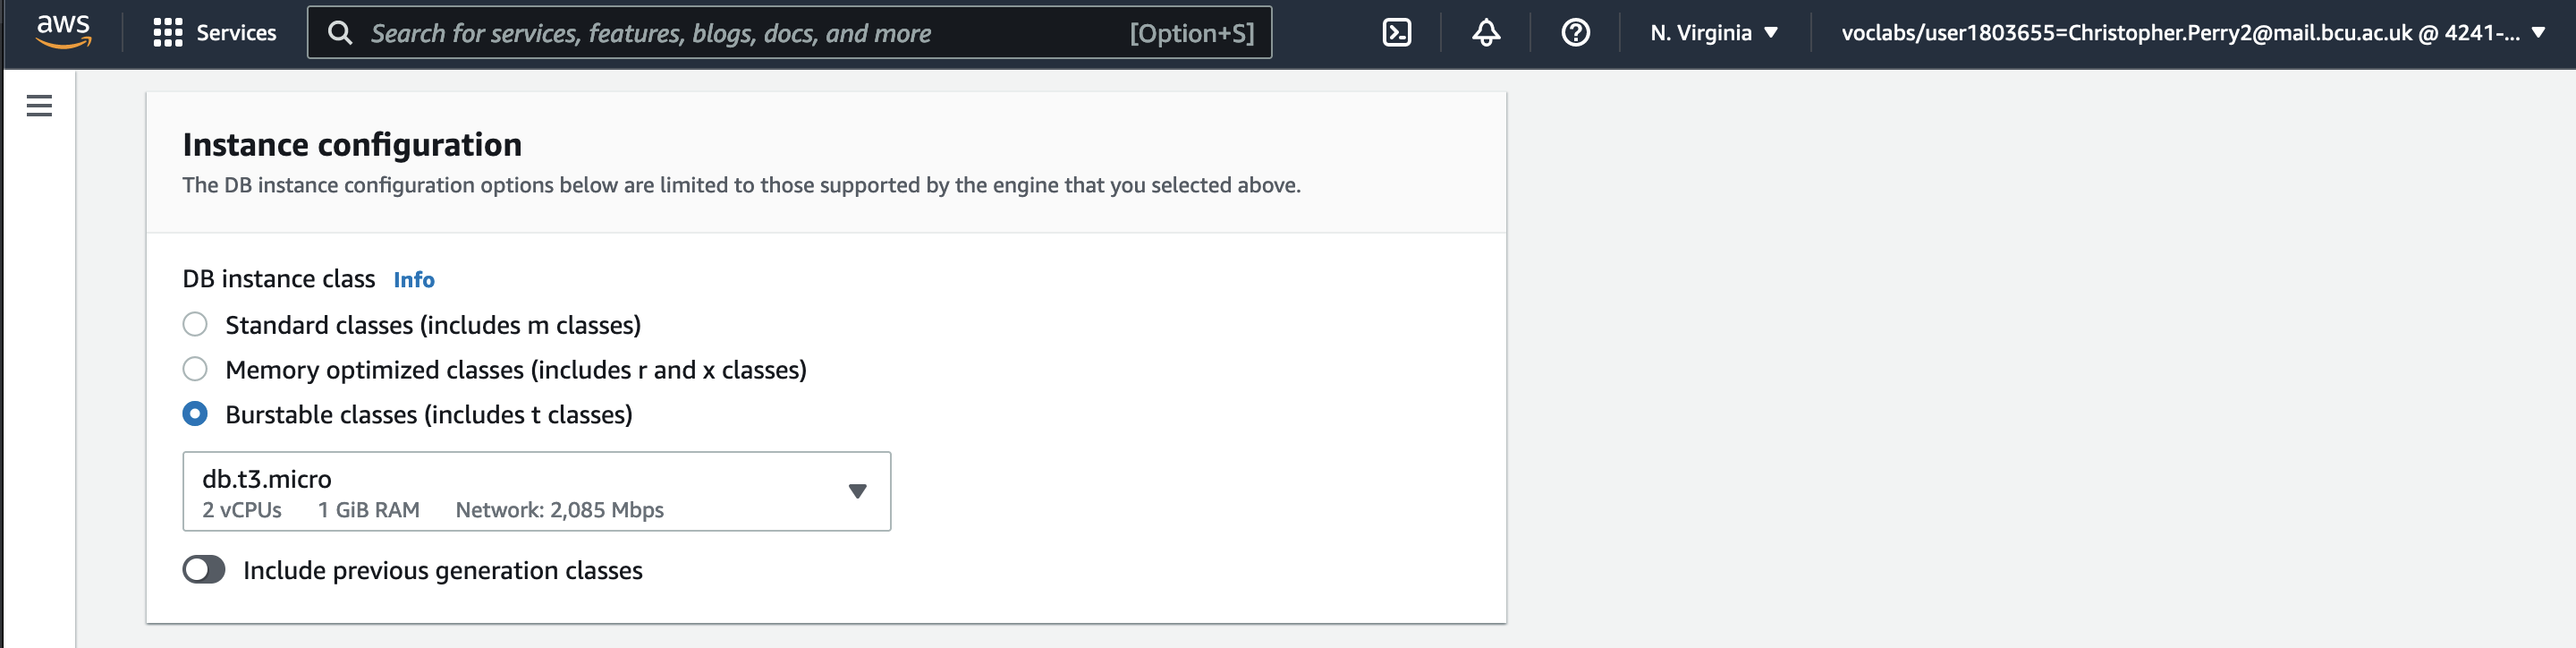
\includegraphics[width=\textwidth]{resources/rds/rds-instance-config.png}
    \caption{Selection of CloudWatch metric for EC2 instance.}
    \label{fig:rds-instance-conf}
\end{figure}

\begin{figure}[!htbp]
    \centering
    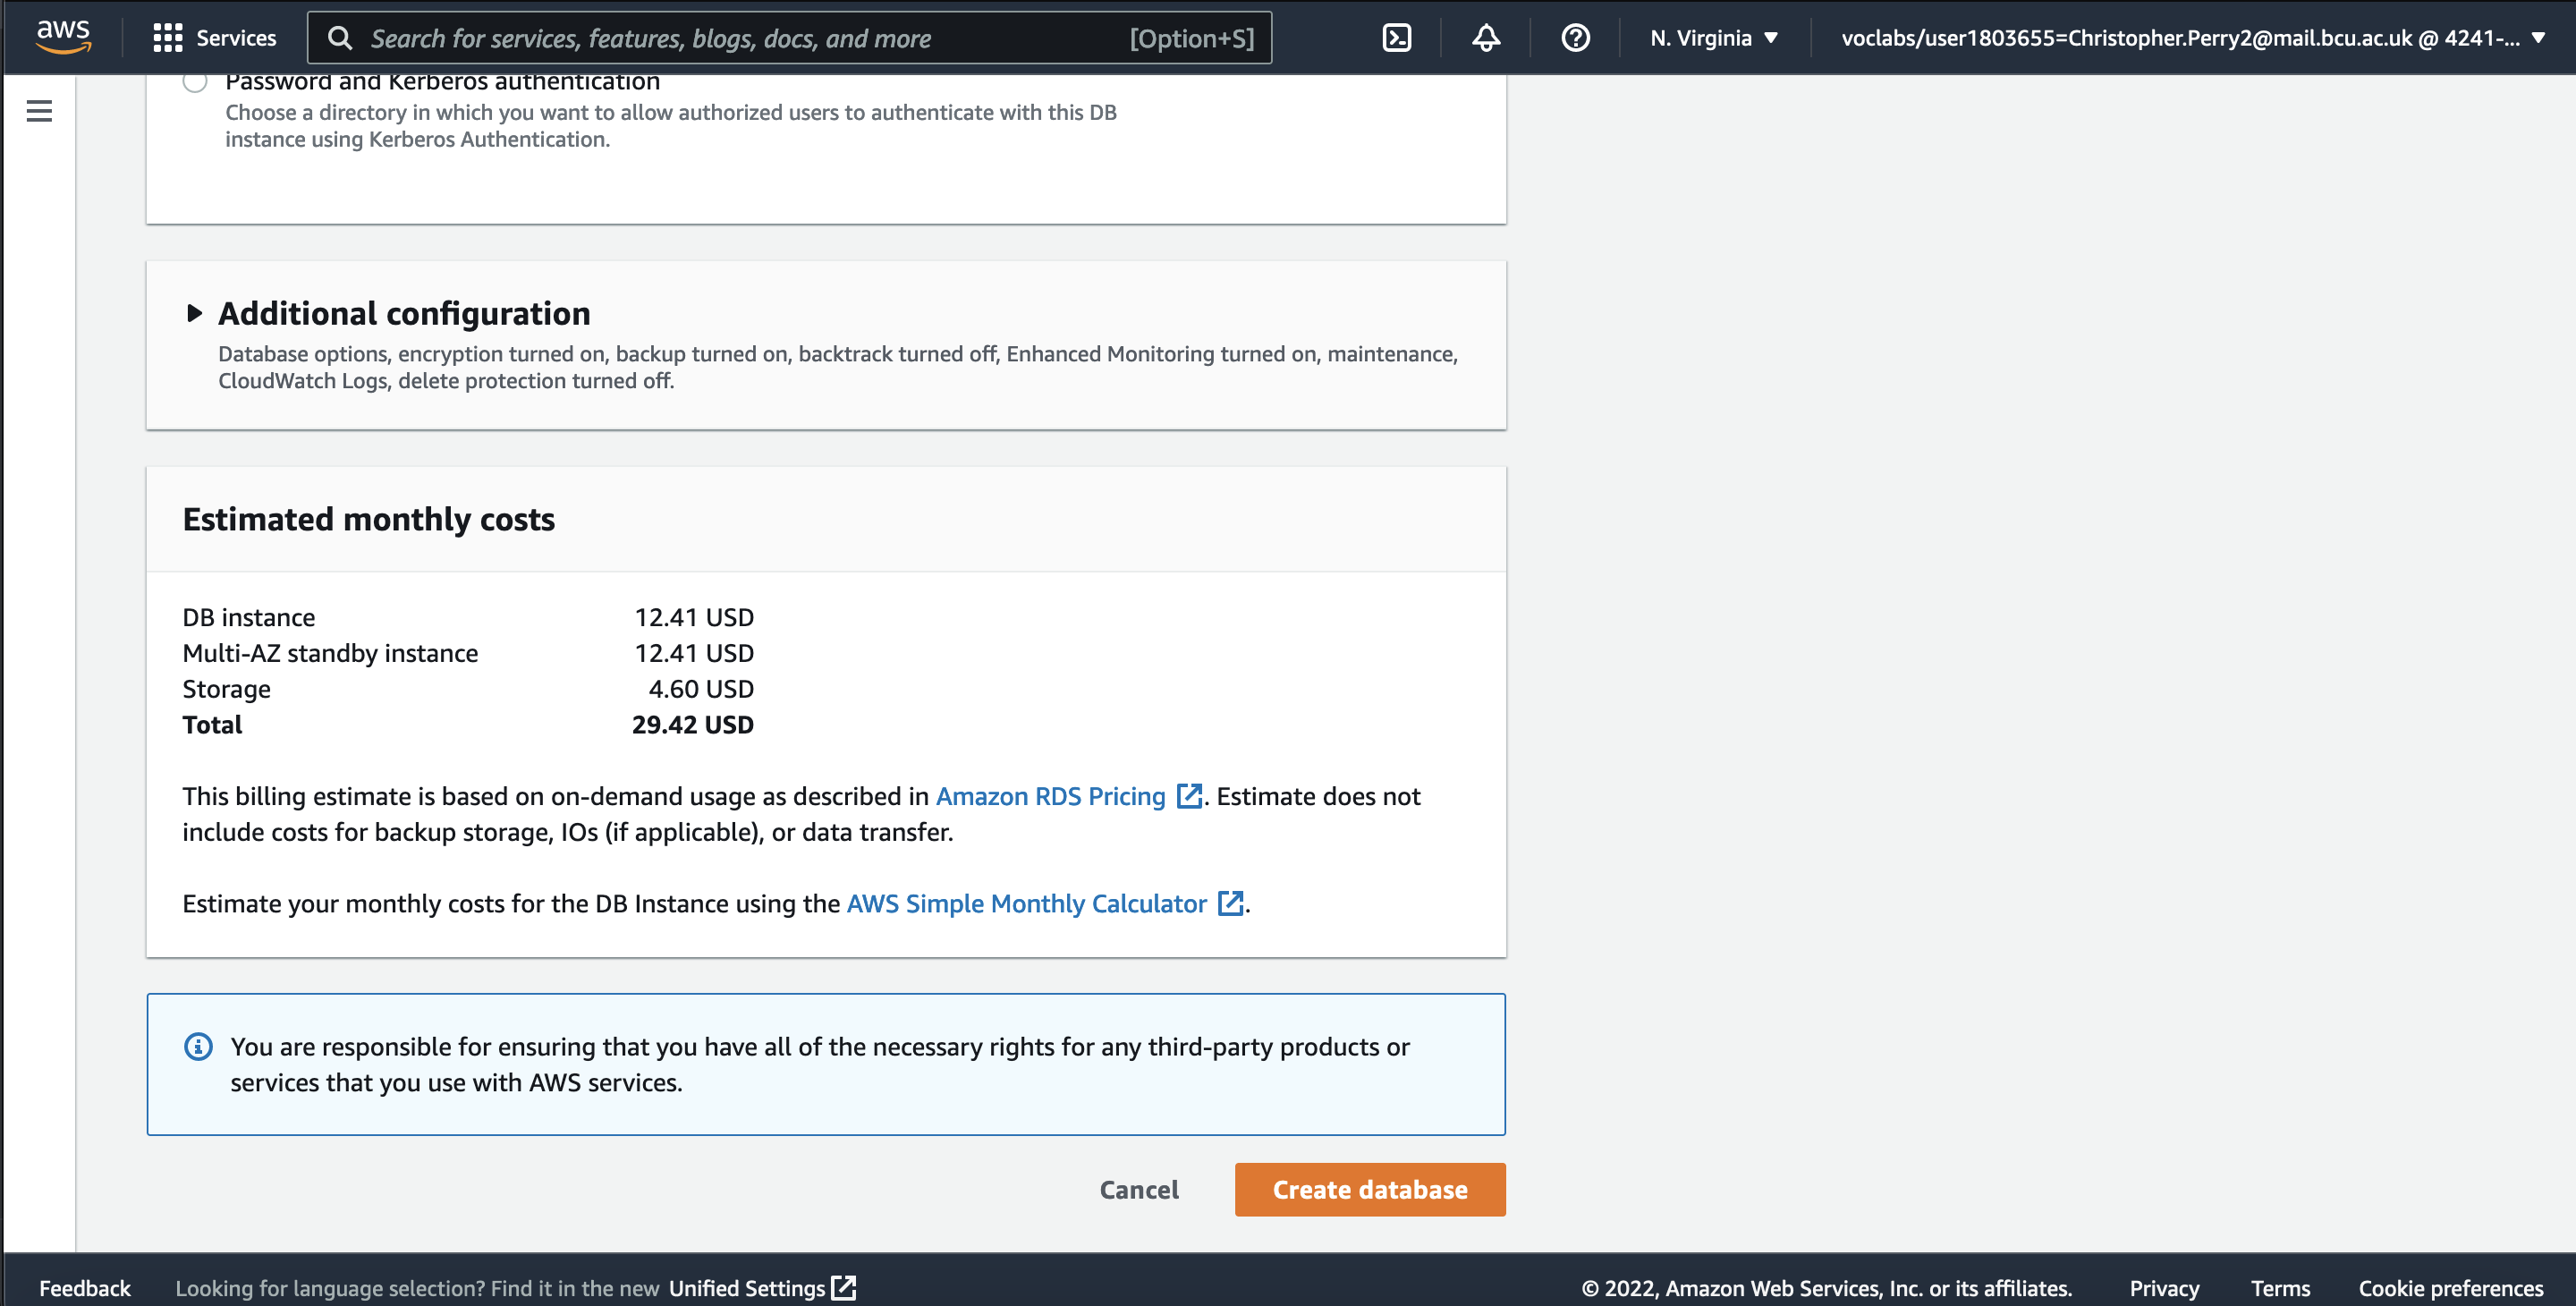
\includegraphics[width=\textwidth]{resources/rds/rds-monthly-costs.png}
    \caption{Selection of CloudWatch metric for EC2 instance.}
    \label{fig:rds-costs}
\end{figure}

\begin{figure}[!htbp]
    \centering
    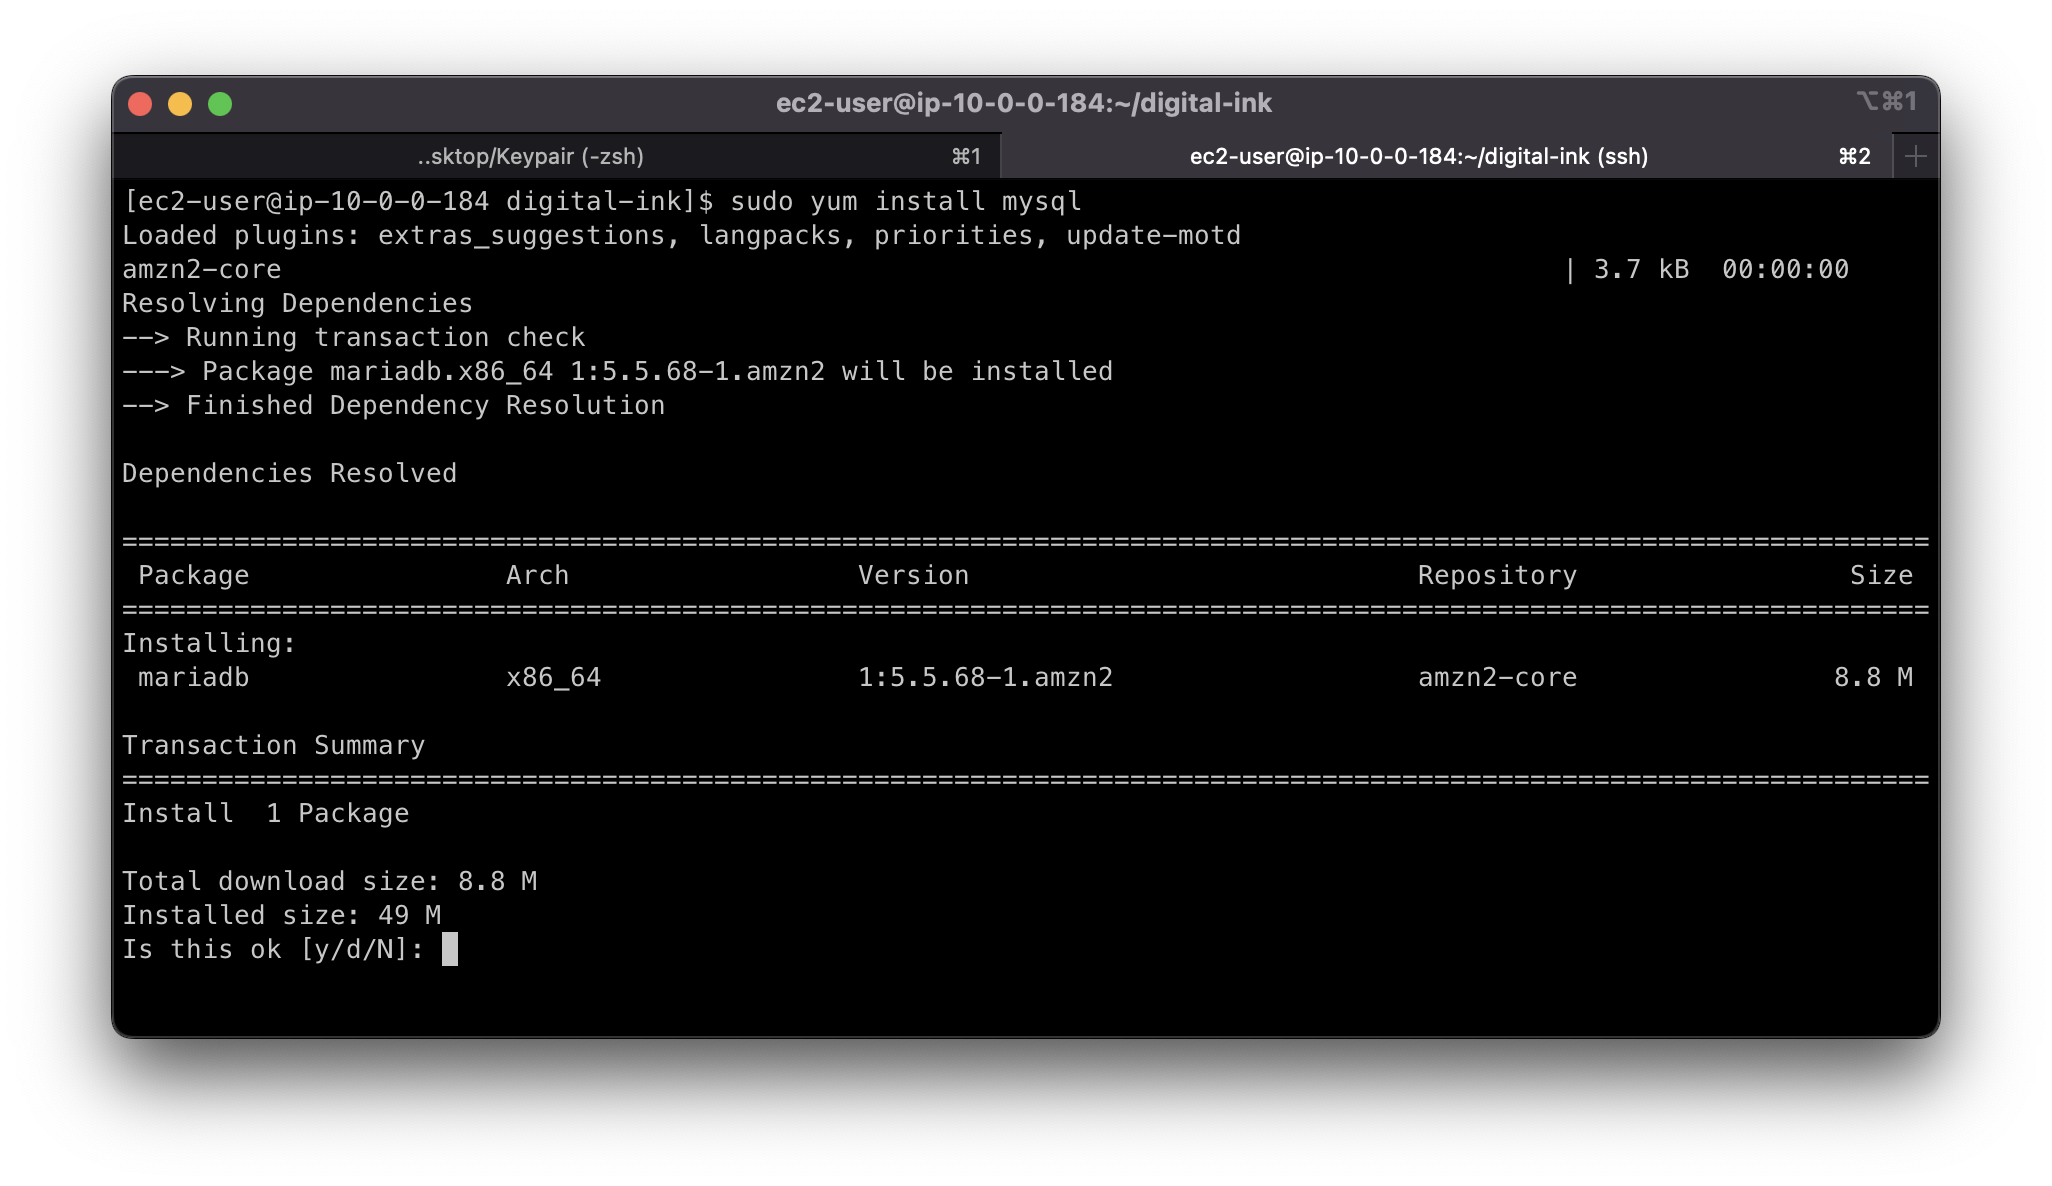
\includegraphics[width=\textwidth]{resources/rds/rds-mysql-install.png}
    \caption{Selection of CloudWatch metric for EC2 instance.}
    \label{fig:rds-msql-install}
\end{figure}

\begin{figure}[!htbp]
    \centering
    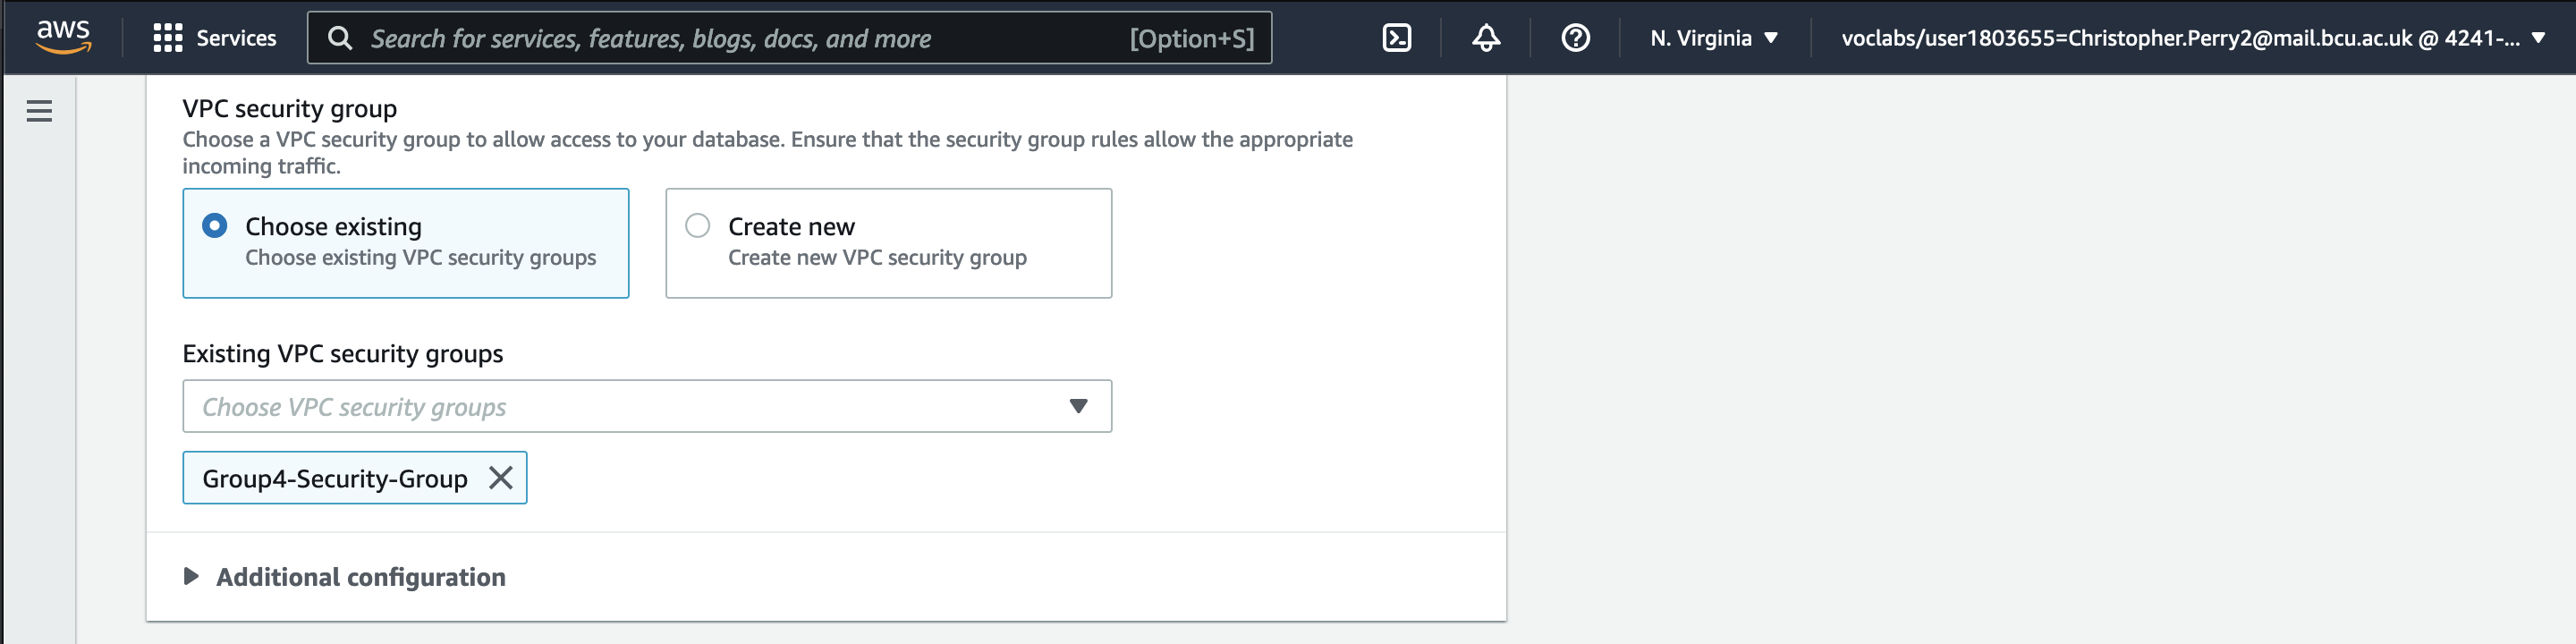
\includegraphics[width=\textwidth]{resources/rds/rds-security-group.png}
    \caption{Selection of CloudWatch metric for EC2 instance.}
    \label{fig:rds-security}
\end{figure}

\begin{figure}[!htbp]
    \centering
    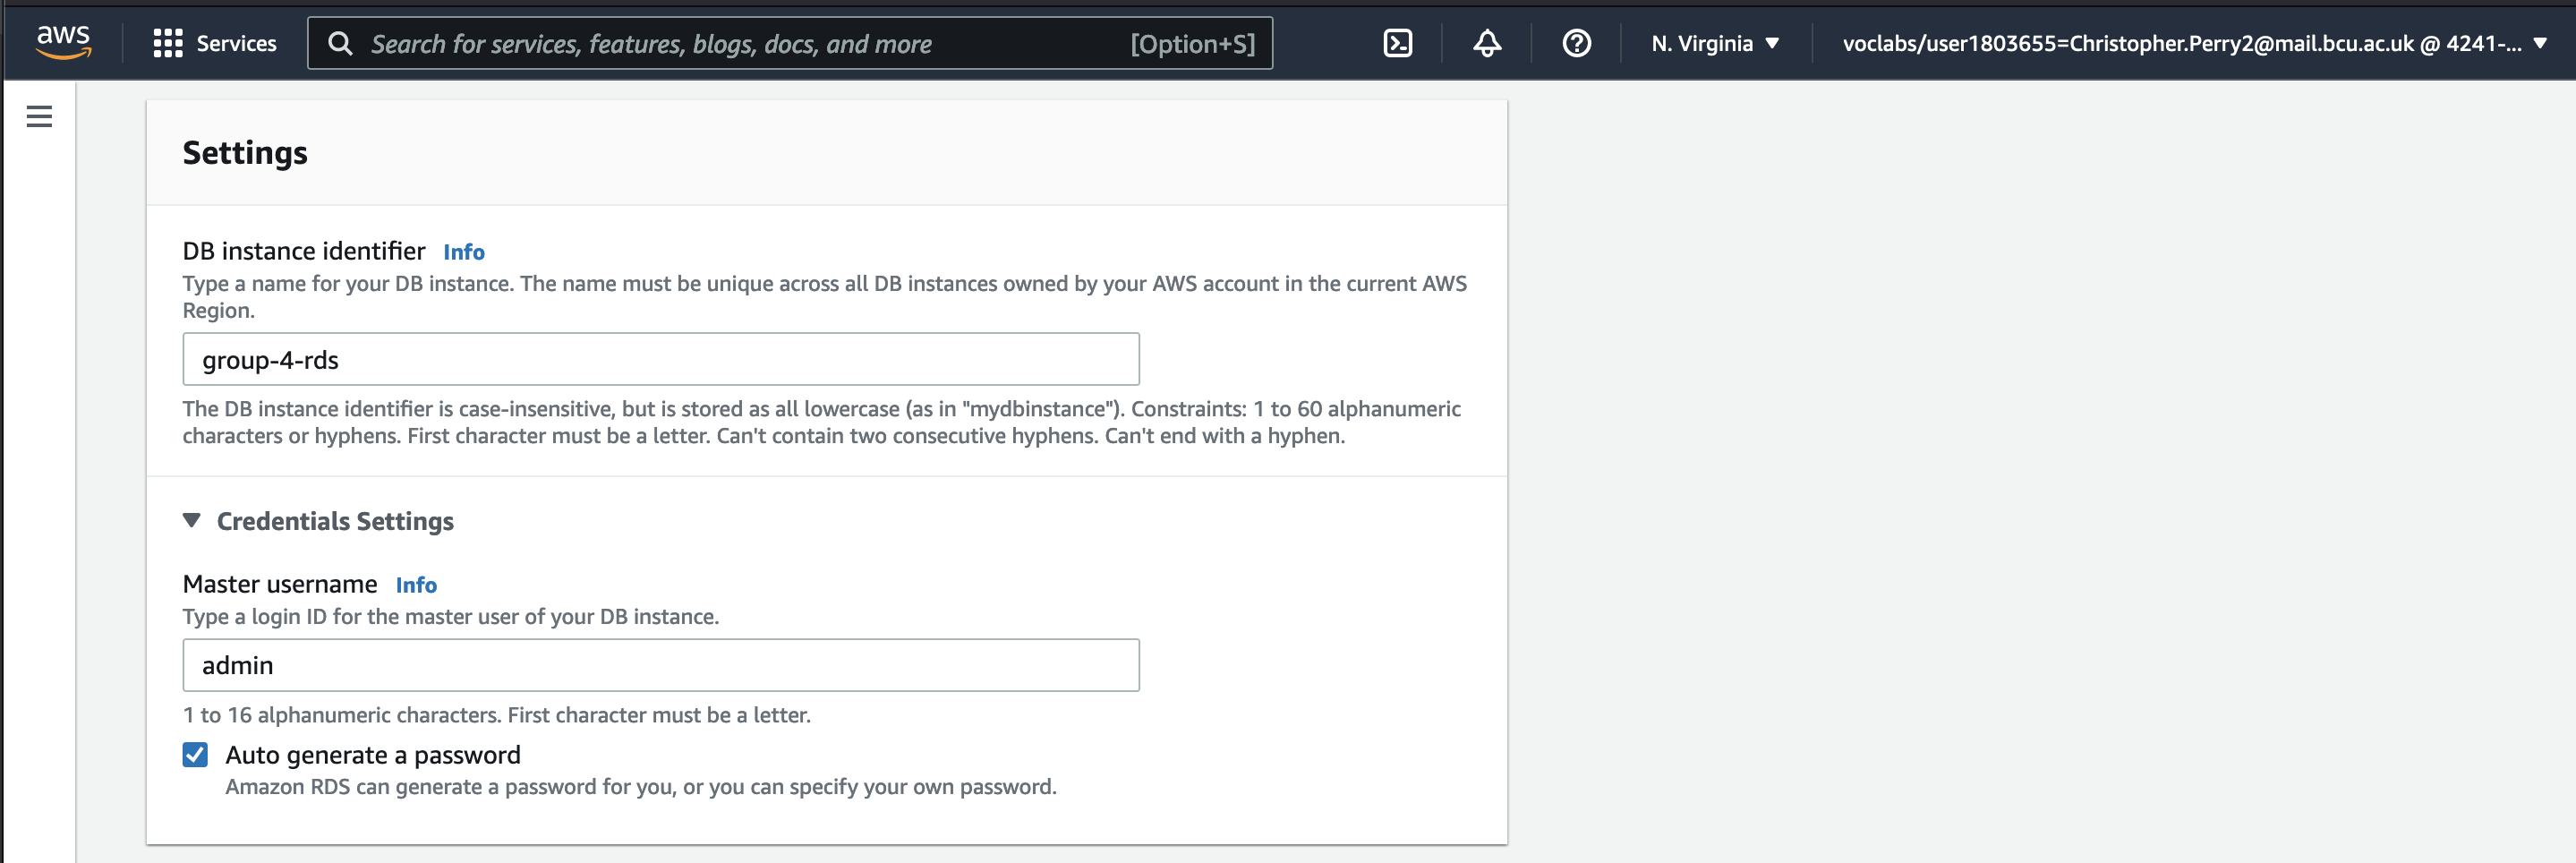
\includegraphics[width=\textwidth]{resources/rds/rds-settings.png}
    \caption{Selection of CloudWatch metric for EC2 instance.}
    \label{fig:rds-settings}
\end{figure}

\begin{figure}[!htbp]
    \centering
    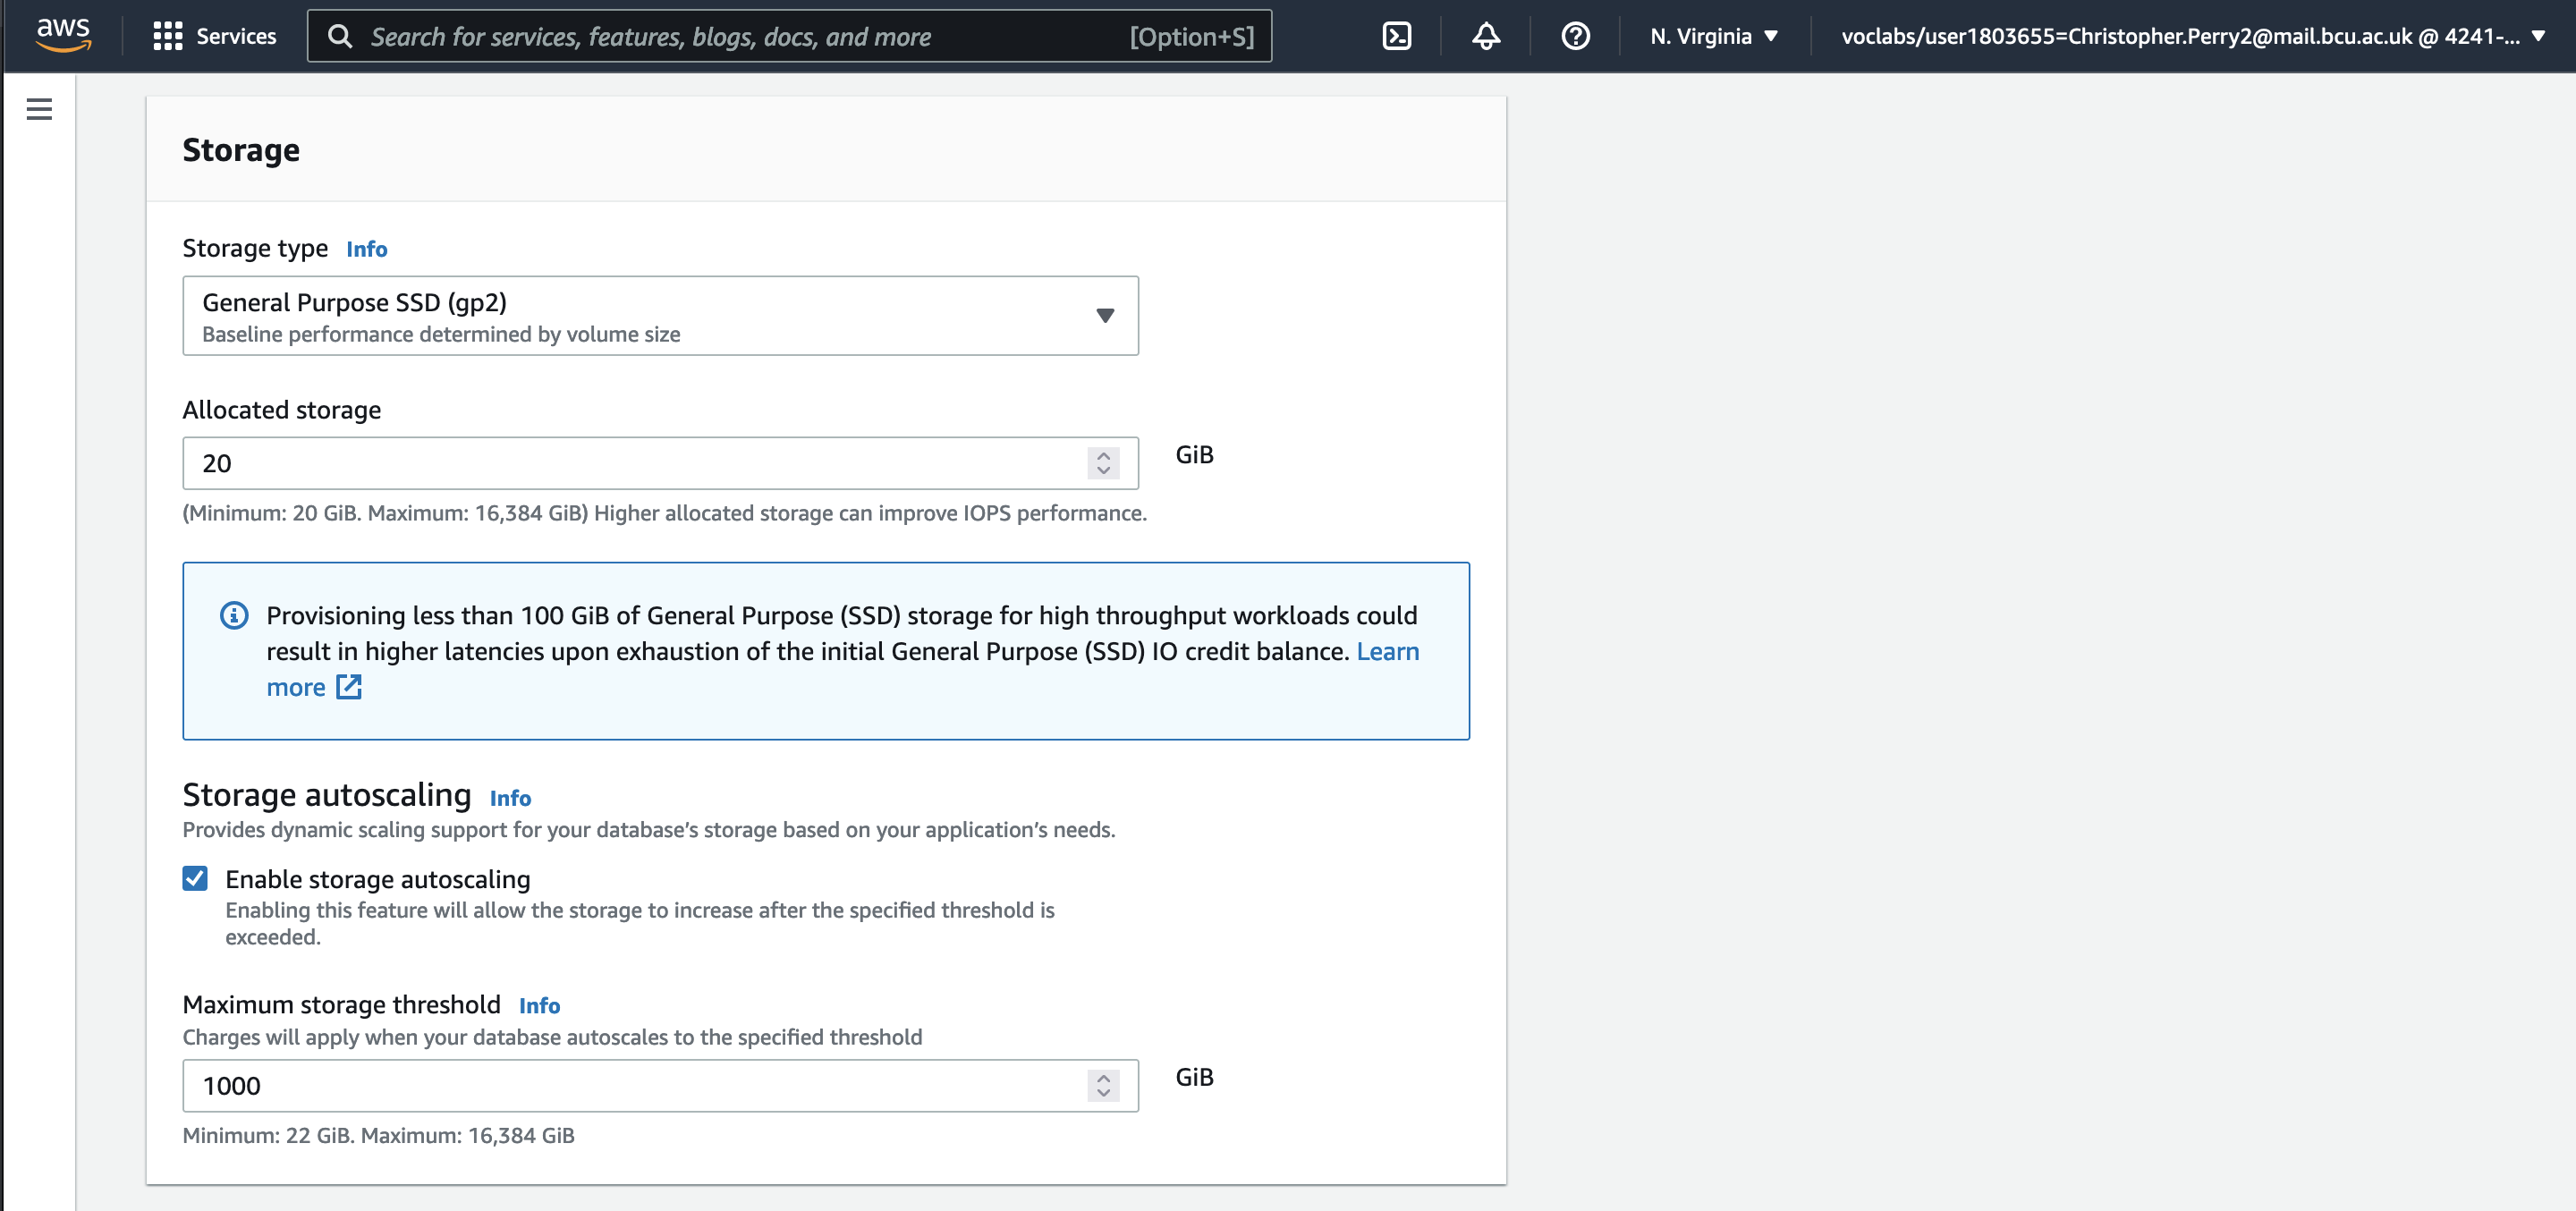
\includegraphics[width=\textwidth]{resources/rds/rds-storage.png}
    \caption{Selection of CloudWatch metric for EC2 instance.}
    \label{fig:rds-storage}
\end{figure}

\begin{figure}[!htbp]
    \centering
    \includegraphics[width=\textwiresources/rds/rds-tables-creation.png}
    \caption{Selection of CloudWatch metric for EC2 instance.}
    \label{fig:rds-tables}
\end{figure}


\begin{figure}[!htbp]
\centering
\includegraphics[width=\textwiresources/rds/rds-templates.png}
\caption{Selection of CloudWatch metric for EC2 instance.}
\label{fig:rds-templates}
\end{figure}